% !BIB TS-program = biber
% !TEX spellcheck = de_DE
%---------------------------------------------------------------------------------
\documentclass[a4paper,11pt,DIV=20,BCOR=10mm] {scrartcl}
%%%%%%%%%%%%%%%%%%%%%%%%%%%%%%%%%%%%%%%%%%%%%%%%%%%%%%%%%%%%%%%%%%%%%%%%%%%%%%%%%%
\newif\ifsolution
%\solutiontrue
\solutionfalse
%%%%%%%%%%%%%%%%%%%%%%%%%%%%%%%%%%%%%%%%%%%%%%%%%%%%%%%%%%%%%%%%%%%%%%%%%%%%%%%%%%
\title{Vereinfachter Blattentwurf}
\subtitle{\ifsolution{\textcolor{red}{Lösung der }}\fi Übung zur Vorlesung \#6 \\ Windenergie Grundlagen}
\author{David Schlipf\\Marcel Schedat}
\date{06.11.2023}
%%%%%%%%%%%%%%%%%%%%%%%%%%%%%%%%%%%%%%%%%%%%%%%%%%%%%%%%%%%%%%%%%%%%%%%%%%%%%%%%%%
\def\StylePath{../WETI-Style/}
\usepackage{\StylePath/WETI-ExerciseDoc}%v1.8
\bibliography{../WETI-Style/PublicationsDavidSchlipf,../ReferencesWEG}
% Additional packages / settings
\sisetup{locale = DE} % comma for floats
%%%%%%%%%%%%%%%%%%%%%%%%%%%%%%%%%%%%%%%%%%%%%%%%%%%%%%%%%%%%%%%%%%%%%%%%%%%%%%%%%%
\begin{document}
% ---------------------------------------
\maketitle 
% ---------------------------------------
% ---------------------------------------
\section*{Blattentwurf nach Betz für die NREL 5MW Windenergieanlage}
% ---------------------------------------
In dieser Übung sollen die Rotorblätter für die NREL 5MW Referenzwindenergieanlage \cite{Jonkman2009a} nach Betz ausgelegt und anschließend mit dem NREL Entwurf verglichen werden. Der Einfachheit halber wird nur das Tragflügelprofil NACA64-A17 verwendet. Für die originalen Rotorblätter werden mehr Profile verwendet.

Bitte folgen Sie den folgenden Schritten
% ---------------------------------------
\begin{enumerate}[noitemsep,label=\alph*)] 
	\item Finden Sie die Entwurfsschnelllaufzahl $\lambda_{\textrm{D}}$, den Rotorradius und die Blattanzahl in \cite{Jonkman2009a}.
	%-----
	\ifsolution{\textcolor{red}{$R=\SI{63}{m}$, $\lambda_{\textnormal{D}}=7.55$, $z=3$.}}\fi
	%=====	
	\item Finden Sie nützliche Entwurfswerte für den Anstellwinkel $\alpha_{\textrm{A}}$ und den Auftriebsbeiwert $c_{\textrm{L}}$. Nutzen Sie dazu die Profildaten in der Datei \file{NACA64_A17.dat}.
	%-----
	\ifsolution{\textcolor{red}{$\alpha_{\textnormal{A}}=\SI{5}{\degree}$, $c_{\textnormal{L}}=1.011$.}}\fi
	%=====	
	\item Berechnen Sie die Verteilung der Verwindung $ \beta(r) $ und der Profiltiefe $ c(r) $ über den Radius an den Positionen aus der Datei \file{NRELOffshrBsline5MW_AeroDyn_Equil_noTwr.dat}.
	%-----
	\ifsolution{
		\newline
		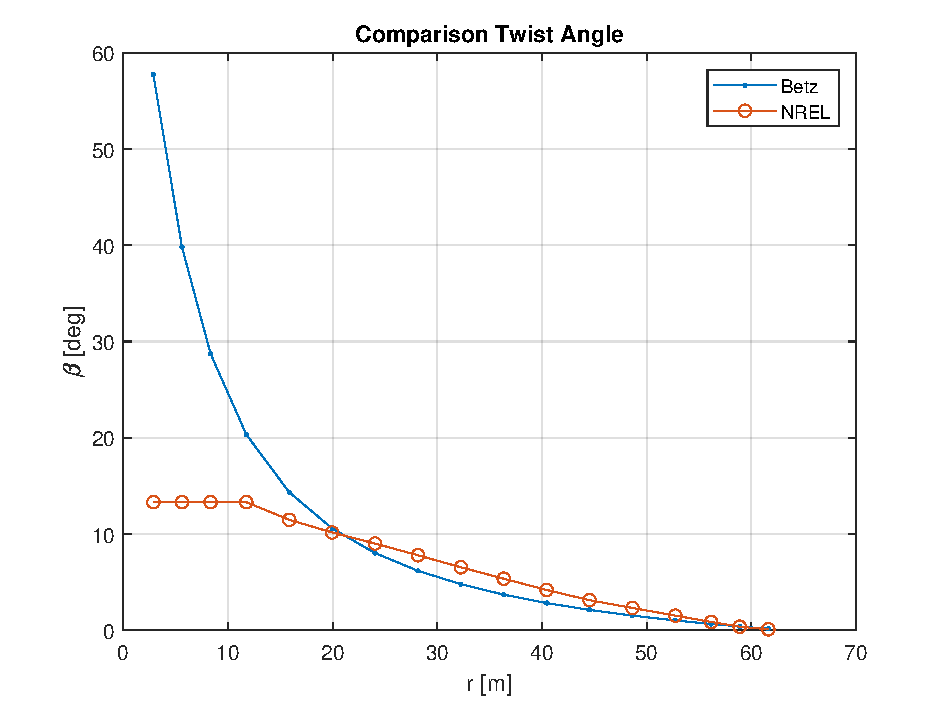
\includegraphics[width=.45\linewidth]{Figures/ComparisonTwistAngle} 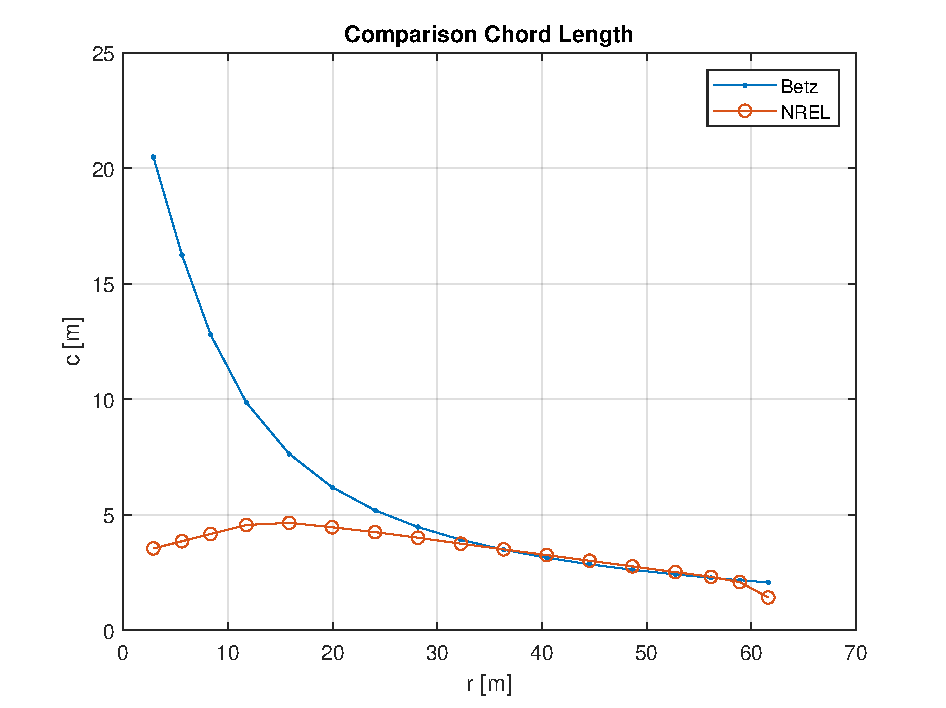
\includegraphics[width=.45\linewidth]{Figures/ComparisonChordLength} 
		\newline
	}\fi
	%=====	
	\item Vergleichen Sie die Werte mit denen aus dem NREL-Design. Was sind die Hauptunterschiede? Wie wurde vermutlich das Blatt ausgelegt?
	%-----
	\ifsolution{\textcolor{red}{Größere Werte für Verwindung und Profiltiefe im Wurzelbereich.}}\fi
	%=====	
\end{enumerate}
% ---------------------------------------
Sie können entweder das Matlabscript \file{WEG_06_Vereinfachter_Blattentwurf_Uebung.m} oder die Exceldatei \file{WEG_06_Vereinfachter_Blattentwurf_Uebung.xlsx} verwenden.

% ---------------------------------------
% bibliography
\printbibliography[title=Quellen]
\end{document} 
